\section{HÌNH HỌC}
\setcounter{ex}{0}


%%Câu 1          
\begin{ex}
	Chọn theo đúng thứ tự xuất hiện của hình $1$, hình $2$, hình $3$.
	\begin{center}
		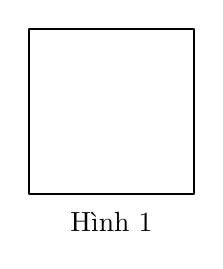
\begin{tikzpicture}[scale=.7,line width=0.8pt, line join=round, line cap=round,>=stealth]
			\draw
			(0,0)rectangle (3,3)
			(1.5,-0.5)node{Hình $1$}
			;
		\end{tikzpicture}\hspace*{1cm}
		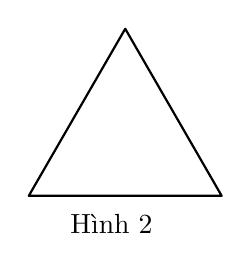
\begin{tikzpicture}[scale=.7,line width=0.8pt, line join=round, line cap=round,>=stealth]
			\draw
			(0,0)--+(0:3.5)--+(60:3.5)--cycle
			(1.5,-0.5)node{Hình $2$}
			;
		\end{tikzpicture}\hspace*{1cm}
		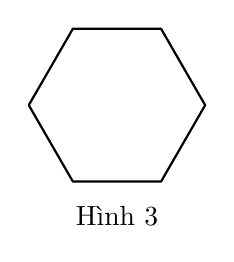
\begin{tikzpicture}[scale=.7,line width=0.8pt, line join=round, line cap=round,>=stealth]
			\path
			(0,0)+(0:1.6)coordinate(A)
			+(60:1.6)coordinate(B)
			+(120:1.6)coordinate(C)
			+(180:1.6)coordinate(D)
			+(240:1.6)coordinate(E)
			+(300:1.6)coordinate(F)
			
			;
			\draw
			(A)--(B)--(C)--(D)--(E)--(F)--cycle
			(0,-2)node{Hình $3$}
			;
		\end{tikzpicture}
	\end{center}
	\choice
	{Tam giác đều – Hình vuông – Lục giác đều}
	{\True Hình vuông – Tam giác đều – Lục giác đều}
	{Hình chữ nhật – Tam giác đều  - Lục giác đều}
	{Hình vuông – Tam giác cân – Lục giác đều}
\end{ex}

%%Câu 5
\begin{ex}%[6H1Y1-1]%[Dự án đề kiểm tra HKI NH23-24- Dương BùiĐức]
	Trong các hình sau đây, hình nào là tam giác đều?
	\begin{center}
		\begin{tikzpicture}[line width=0.8pt,scale=0.8]
			\def\h{2.5}
			\def\goc{60}
			\path
			(0,0) coordinate (B)
			+(\goc:2*\h) coordinate (b)
			++(0:\h) coordinate (C)
			+(180-\goc:\h) coordinate (c)
			($(B)!1/2!(C)$) coordinate (H)
			(intersection of B--b and C--c) coordinate (A)
			;
			\pgfresetboundingbox
			\draw 
			(A)--(B)--(C)--cycle
			;
			\foreach \x/\y/\z in {
				C/B/\times,
				A/B/\times,
				A/C/\times
			}\path (\x)--(\y) node[pos=0.5,sloped]{$\z$};
			\path (current bounding box.south) node[below]{Hình 1};
		\end{tikzpicture} \hfil
		\begin{tikzpicture}[line width=0.8pt,scale=0.8]
			\def\h{2.5}
			\def\goc{90}
			\path
			(0,0) coordinate (B)
			+(\goc:\h) coordinate (A)
			++(0:1.3*\h) coordinate (C)
			;
			\pgfresetboundingbox
			\draw 
			(A)--(B)--(C)--cycle
			;
			
			\foreach \a/\b/\c in
			{A/B/C}{\draw pic[draw,angle radius=3mm] {right angle = \a--\b--\c};}
			\path (current bounding box.south) node[below]{Hình 2};
		\end{tikzpicture} \hfil
		\begin{tikzpicture}[line width=0.8pt,scale=0.8]
			\def\h{2}
			\def\goc{70}
			\path
			(0,0) coordinate (B)
			+(\goc:2*\h) coordinate (b)
			++(0:\h) coordinate (C)
			+(180-\goc:\h) coordinate (c)
			($(B)!1/2!(C)$) coordinate (H)
			(intersection of B--b and C--c) coordinate (A)
			;
			\pgfresetboundingbox
			\draw 
			(A)--(B)--(C)--cycle
			;
			\path (current bounding box.south) node[below]{Hình 3};
		\end{tikzpicture} \hfil
		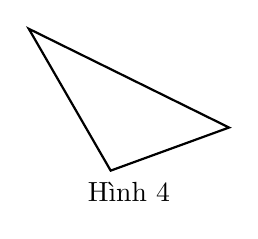
\begin{tikzpicture}[line width=0.8pt,scale=0.8]
			\def\h{2}
			\def\goc{70}
			\path
			(0,0) coordinate (B)
			+(20:\h) coordinate (C)
			+(120:1.3*\h) coordinate (A)
			;
			\pgfresetboundingbox
			\draw 
			(A)--(B)--(C)--cycle
			;
			\path (current bounding box.south) node[below]{Hình 4};
		\end{tikzpicture}
	\end{center}
	\choice
	{\True Hình 1}
	{Hình 2}
	{Hình 3}
	{Hình 4}
\end{ex}

\begin{ex}%[6H1Y1-1] 
	\immini{
		Tam giác ABC được gọi là tam giác đều nếu
		\choice
		{Mỗi góc đỉnh $A, B, C$ có số đo bằng $90^\circ$}
		{Mỗi góc đỉnh $A, B, C$ có số đo bằng $80^\circ$}
		{\True Mỗi góc đỉnh $A, B, C$ có số đo bằng $60^\circ$}
		{Mỗi góc đỉnh $A, B, C$ có số đo bằng $30^\circ$}
	}{
		\begin{tikzpicture}[line join = round, line cap = round,line width=0.8pt,>=stealth,font=\footnotesize,scale=1] 
			\def\a{2.5}
			\def\goc{60}
			\coordinate[label = left:$B$] (B) at (0,0); 
			\coordinate[label = right:$C$] (C) at ($(B)+(\a,0)$); 
			\coordinate[label = above:$A$] (A) at ($(B)+(\goc:\a)$); 
			\draw (A)--(B)--(C)--cycle; 
			\foreach \x in {A,B,C} \fill[black] (\x) circle (1.5pt);
		\end{tikzpicture}
	}
\end{ex}

\begin{ex}%[6H1B4-1]
	Hình thang cân có các tính chất nào sau đây? 
	\choice
	{Có hai đường chéo vuông góc}
	{Có bốn cạnh bằng nhau}	
	{Có bốn cạnh song song với nhau}
	{\True Có hai góc kề một đáy bằng nhau}
\end{ex}

%%Câu 2
\begin{ex} 
	Yếu tố nào sau đây không phải của hình bình hành?
	\choice
	{ Hai cặp cạnh đối diện song song}
	{Hai cặp cạnh đối diện bằng nhau}
	{\True Hai đường chéo bằng nhau}
	{Hai đường chéo cắt nhau tại trung điểm của mỗi đường}
\end{ex}     

%%Câu 6
\begin{ex}
	Hình thoi là
	\choice
	{\True Hình có bốn cạnh bằng nhau}
	{Hình có bốn cạnh bằng nhau và bốn góc vuông}
	{Hình có hai đường chéo bằng nhau}
	{Hình có bốn góc bằng nhau và bằng góc vuông}
\end{ex}

%%Câu 9
\begin{ex}
	Khẳng định nào sau đây là đúng? Trong hình chữ nhật:
	\choice
	{Hai đường chéo song song với nhau}
	{\True Bốn góc bằng nhau}
	{Hai đường chéo không bằng nhau}
	{Bốn góc không bằng nhau}
\end{ex}

\begin{ex} 
	Ba đường chéo chính của lục giác đều $A B C D E F$ là
	\choice
	{$A B$, $C D$, $A C$}
	{\True $A D$, $F C$, $E B$}
	{$AB$, $CD$, $EF$}
	{$F E$, $E D$, $D C$}	
\end{ex}


%%% câu 7
\begin{ex}%[6H1Y1-1] 
	\immini{
		Cho hình vuông MNPQ, khẳng định nào sau đây \textbf{đúng}?
			\choice
		{MN và MQ song song}
		{MN và MP song song}
		{MQ và PQ song song}
		{\True MN và PQ song song}
	}{
		\begin{tikzpicture}[scale=1,line width=0.8pt,line join=round,>=stealth]
			\def\a{2} 
			\path (0,0) coordinate (M)
			(M)+(0:\a) coordinate (N)
			(N)+(-90:\a) coordinate (P)
			(M)+(-90:\a) coordinate (Q)
			;
			\draw (M)--(N)--(P)--(Q)--(M);
			\foreach \x/ \goc in {M/135,N/45,P/-45,Q/-135}  \fill (\x) circle (1.5pt) ($(\x)+(\goc:3.5mm)$) node {$\x$};
		\end{tikzpicture}
	}
\end{ex}

\begin{ex}%[6H1Y1-7] 
	Cho tam giác đều $ABC$ với $AB=17$ cm. Độ dài cạnh $BC$ là
	\choice
	{\True $17$ cm}
	{$7{,}5$ cm}
	{$30$ cm}
	{$5$ cm}
\end{ex}

%%Câu 10
\begin{ex} Hình thoi có độ dài hai đường chéo lần lượt là 15 cm, 20 cm thì diện tích hình thoi là:
	
	\choice
	{300}
	{\True 150}
	{70}
	{75}
\end{ex}

\begin{ex}
	Cho hình chữ nhật ABCD có AB= 3cm. Độ dài cạnh AD lớn hơn cạnh AB 4 cm. Chu vi hình chữ nhật ABCD là bao nhiêu cm.
	\choice
	{10}
	{\True 20}
	{21}
	{14}
	
\end{ex}

\begin{ex}\immini[thm]{
		Mỗi viên gạch hình vuông có cạnh $20$ cm. Tính chu vi hình vuông ghép bởi $4$ viên gạch hoa như hình vẽ dưới đây.
		\hfill
		\choice
		{$1600$ cm$^2$}
		{$1600$ cm}
		{$160$ cm$^2$}
		{\True $160$ cm}	
	}{
		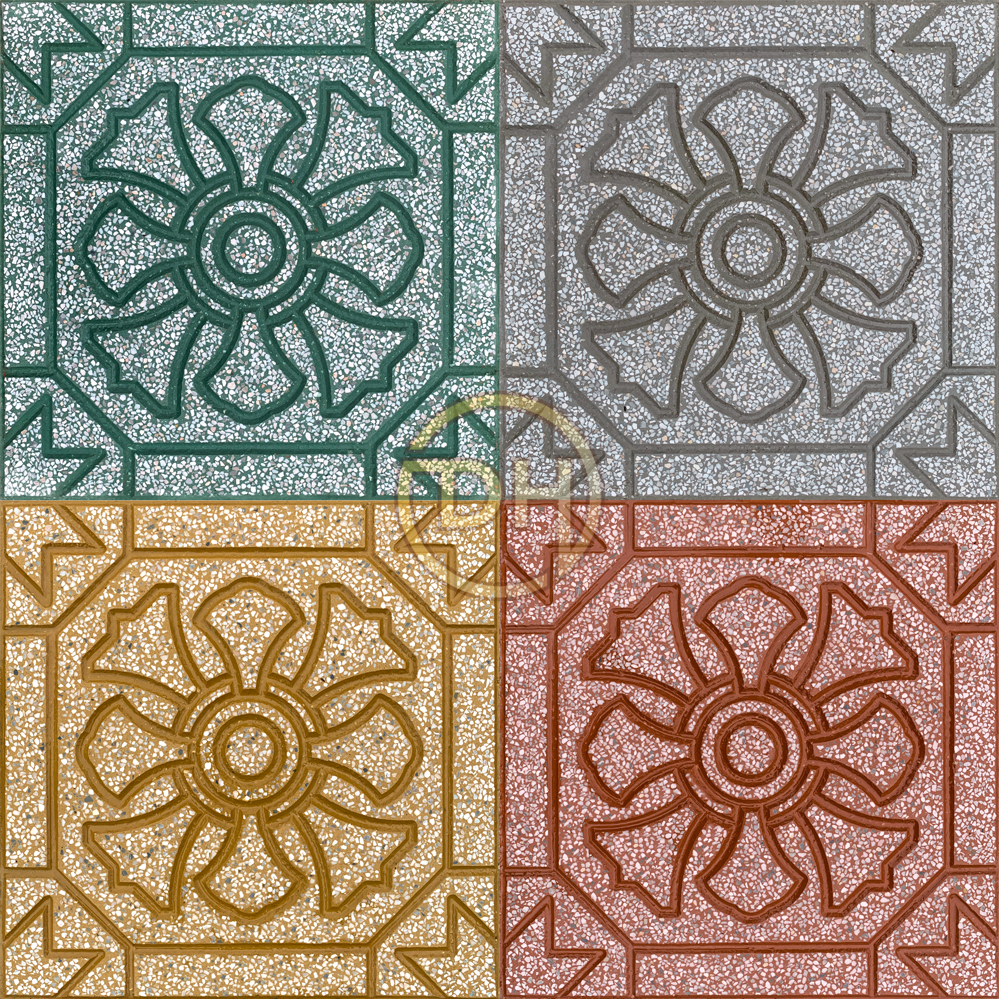
\includegraphics[scale=0.12]{data/Hình/C25_TN_HH}
	}
	
\end{ex}

\begin{ex}%Câu 8%[6H1Y1-4]% 
	Một hình vuông có diện tích $169 $ cm$^2$. Độ dài cạnh hình vuông là
	\choice
	{$10$ cm}
	{\True $13$ cm}
	{$36$  cm}
	{$24$ cm}
	
\end{ex}

%15
\begin{ex}%[6H1Y1-1] 
	\immini{
		 Khung của một bàn học làm bằng sắt được thiết kế như hình bên dưới. Mặt bàn là hình thang cân có đáy lớn dài $1200$ mm, đáy bé dài $600$ mm, cạnh bên dài $500$ mm. Mỗi chân bàn dài $730$ mm. Tính tổng độ dài các thanh sắt cần sử dụng để làm bàn học trên
		 	\choice
		 {\True $5720$ mm}
		 {$5220$ mm}
		 {$3030$ mm}
		 {$2530$ mm}
	}{
	%	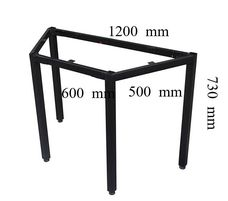
\includegraphics[width=4cm]{data/Hình/C6_HH_TN}
			\begin{tikzpicture}[scale=1,line join=round,line cap=round,>=stealth]
			\def\a{1.2} 
			
			\path
			(0,0)coordinate(O)
			(-15:1.8*\a)coordinate(A)
			(72:0.8*\a)coordinate(D)
			(D)++(-8:3.2*\a)coordinate(C)
			(A)++(-90:1.75*\a)coordinate(A')
			(D)++(-85:1.75*\a)coordinate(D')
			(C)++(-95:1.75*\a)coordinate(C')
			(O)++(-85:1.75*\a)coordinate(O')
			($(O)!0.62!(A)$) node[below, rotate=-15,yshift=-0.1 cm]{$600$ mm}
			($(D)!0.5!(C)$) node[below, rotate=-8,yshift=-0.1 cm]{$1200$ mm}
			($(A)!0.45!(C)$) node[below, rotate=28,yshift=-0.1 cm]{$500$ mm}
			($(C)!0.62!(C')$) node[below, rotate=-95,yshift=0.7 cm]{$730$ mm}
			;
			\draw [line width=3pt]
			(O)--(A)-- (C)--(D)--(O)
			
			(A)--(A') (O)--(O') (C)--(C') (D)--(D')
			; 
			
			%%%% Hiển thị tên điểm
			%	\foreach \x/\g in {A/-40,D/90,C/90,O/-130
				%	}\draw[fill=white](\x)circle(1.5pt)+(\g:.3)node{$\x$};
		\end{tikzpicture}
	}
\end{ex}

%%Câu 18:
\begin{ex}
	\immini[thm]{
		Tính diện tích phần gạch sọc trong hình sau biết các kích thước như hình vẽ:
		\choice
		{$56$ m$^2$}
		{$42$ m$^2$}
		{$36$ m$^2$}
		{\True $28$ m$^2$}
	}{
	\begin{tikzpicture}[scale=1,line width=0.8pt,line join=round,>=stealth]
		\def\sc{2.5} 
		\path (0,0) coordinate (A)
		(A)+(0:14/\sc) coordinate (B)
		(B)+(-90:4/\sc) coordinate (C)
		(C)+(180:14/\sc) coordinate (D)
		(C)+(180:7/\sc) coordinate (G)node[below]{14 m}
		(A)+(0:5/\sc) coordinate (E)
		(A)+(0:9/\sc) coordinate (F)
		;
		\filldraw[pattern=north east lines] (D)--(A)node[midway,left]{4 m}--(B)--(C)--(G)--(D);
		\draw[fill=white] (D)--(E)--(G)--(F)--(C)--cycle;
		\draw (C)--(G)node[midway]{\small ||}--(D)node[midway]{\small ||};
	\end{tikzpicture}	
	}

\end{ex}



%%=====Câu 46
\begin{ex}%[6H1B2-4] 
	Một hình thoi có diện tích bằng $24$ cm$^2$. Biết độ dài một cạnh đường chéo bằng $6$ cm, tính độ dài đường chéo còn lại của hình thoi đó.
	\choice
	{$4$ cm}
	{$16$ cm}
	{$12$ cm}
	{\True $8$ cm}
\end{ex}


%%=====Câu 48
\begin{ex}\immini[thm]{
	Tính diện tích và chu vi phần in đậm trong hình dưới dây gần nhất với kết quả nào?
	\choice
	{16,8 cm$^2$; 14,9 cm$^2$}
	{7,4 cm$^2$; 14,9 cm$^2$}
	{\True 16,8 cm$^2$; 11,7 cm}
	{ 7,4 cm$^2$; 11,7 cm}	
	}{
		%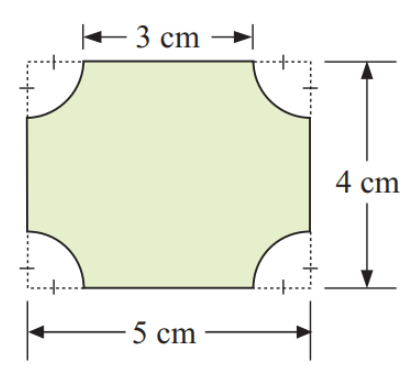
\includegraphics[scale=0.5]{data/Hình/C48_TN_HH}
		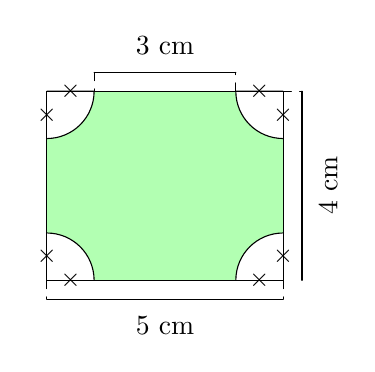
\begin{tikzpicture}[scale=1,line join=round,line cap=round,>=stealth]
		\def\a{0.6} 
		
		
		\path
		(0,0)coordinate(O)
		(90:1*\a)coordinate(A)
		(90:3*\a)coordinate(B)
		(90:4*\a)coordinate(C)
		
		(0:1*\a)coordinate(D)
		(0:4*\a)coordinate(E)
		(0:5*\a)coordinate(F)
		
		(F)++(90:1*\a)coordinate(G)
		(F)++(90:3*\a)coordinate(H)
		(F)++(90:4*\a)coordinate(K)
		
		(C)++(0:1*\a)coordinate(I)
		(C)++(0:4*\a)coordinate(J)
		(C)++(0:5*\a)coordinate(M)
		
		(I)++(90:0.4*\a)coordinate(i)
		(J)++(90:0.4*\a)coordinate(j)
		
		(O)++(-90:0.4*\a)coordinate(o)
		(F)++(-90:0.4*\a)coordinate(f)
		
		(K)++(0:0.4*\a)coordinate(k)
		(F)++(0:0.4*\a)coordinate(f')
	
		;
		
		
		\draw[dashed, fill=green!30] (O)--(C)--(K)--(F)--(O);
		
		\draw [fill=white]  
		(C)--++(0:1*\a) arc (0:-90:1*\a)-- cycle
		(K)--++(180:1*\a) arc (180:270:1*\a)-- cycle
		(O)--++(0:1*\a) arc (0:90:1*\a)-- cycle
		(F)--++(90:1*\a) arc (90:180:1*\a)-- cycle
		
		;  
		
		\fill[white]
		(B)--(C)--(I)--(B)(K)--(H)--(J)--(K)(O)--(A)--(D)--(O)(E)--(G)--(F)--(E);
		
		\draw    
		(A)--(B)--(C)node[midway]{\small $\times$}--(I)node[midway]{\small $\times$}--(J)--(K)node[midway]{\small $\times$}-- (H)node[midway]{\small $\times$}--(G)--(F)node[midway]{\small $\times$}--(E)node[midway]{\small $\times$}-- (D)--(O)node[midway]{\small $\times$}--(A)node[midway]{\small $\times$};
		\draw[dashed](i)--(I) (J)--(j) (O)--(o) (K)--(k) (F)--(f);
		\draw[>=stealth]
		(i) -- (j)node[midway,above, rotate=0,yshift=0.1 cm]{$3$ cm}
		(o) -- (f)node[midway,below, rotate=0,yshift=-0.1 cm]{$5$ cm}
		(k) --(f')node[midway,below, rotate=90,yshift=-0.1 cm]{$4$ cm}
		;
		
		%%%% Hiển thị tên điểm
		%		\foreach \x/\g in {A/-40,O/90,C/90,D/9,B/9,E/9,F/9,G/9,H/9,K/9,I/9,J/9,K/9			}\draw[fill=white](\x)circle(1.5pt)+(\g:.3)node{$\x$};
	\end{tikzpicture}
	}
	
\end{ex}


	
%%=====Câu 49

\begin{ex}\immini[thm]{
	Hãy tính diện tích phần tô đậm, cho biết diện tích đó gần nhất với kết quả nào sau đây:
	
	\choice
	{\True 6,6 cm$^2$}
	{3,6 cm$^2$}
	{4,4 cm$^2$}
	{7,4 cm$^2$}	
	}{
		%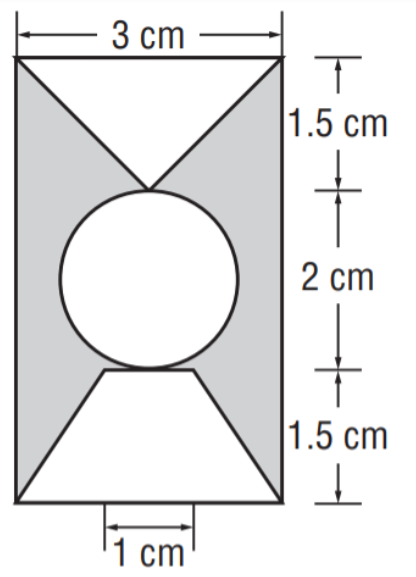
\includegraphics[scale=0.4]{data/Hình/C49_TN_HH}
		\begin{tikzpicture}[scale=1,line join=round,line cap=round,>=stealth]
			\def\a{0.82} 
			
			\path
			(0,0)coordinate(O)
			(0:3*\a)coordinate(A)
			(90:5*\a)coordinate(D)
			(D)++(0:3*\a)coordinate(C)
			
			($(D)!0.5!(C)$) coordinate(b)
			(b)++(-90:1.5*\a)coordinate(B)
			(b)++(-90:2.5*\a)coordinate(E)
			
			($(O)!0.5!(A)$) coordinate(f)
			(f)++(90:1.5*\a)coordinate(g)
			(g)++(0:0.5*\a)coordinate(G)
			(g)++(0:-0.5*\a)coordinate(H)
			%
			(D)++(90:0.4*\a)coordinate(k)
			(C)++(90:0.4*\a)coordinate(f')
			(C)++(0:0.4*\a)coordinate(i)
			(B)++(0:1.9*\a)coordinate(j)
			(g)++(0:1.9*\a)coordinate(o)
			(A)++(0:0.4*\a)coordinate(m)
			(B)++(0:2.1*\a)coordinate(j')
			(g)++(0:2.1*\a)coordinate(o')
			(H)++(-90:1.63*\a)coordinate(p)
			(G)++(-90:1.63*\a)coordinate(q)
			;
			
			\draw[ fill=green!30]
			(O)--(A)--(C)--(D)--(O);
			\draw [fill=white]
			(D)--(B)--(C)--(D)
			(O)--(H)--(G)--(A)
			(E) circle (\a cm)
			; 
			\draw[>=stealth]
			(i) -- (j)node[midway,below , rotate=90,yshift=-0.12 cm]{$1.5$ cm}
			(o) -- (m)node[midway,below, rotate=90,yshift=-0.12 cm]{$1.5$ cm}
			(k) --(f')node[midway,below, rotate=0,yshift=0.55 cm]{$3$ cm}
			(j') --(o')node[midway,below, rotate=90,yshift=-0.12 cm]{$2$ cm}
			(p) --(q)node[midway,below, rotate=0,yshift=-0.12 cm]{$1$ cm}
			;
			\draw[dashed](C)--(i) (B)--(j') (g)--(o')(A)--(m) (D)--(k)(C)--(f') (H)--(p) (G)--(q);
			%%%% Hiển thị tên điểm
		%		\foreach \x/\g in {A/-40,D/90,C/90,O/-130,E/9,B/9,b/9,f/9,G/9,H/9,g/9,k/9,p/9,q/9,j'/9,o'/9,f'/9,i/9,j/9,m/9,o/9	}\draw[fill=white](\x)circle(1.5pt)+(\g:.3)node{$\x$};
		\end{tikzpicture}
	}
		
\end{ex}

\begin{ex}%[6H1B2-4] 
	Bác Hòa uốn một sợi dây thép thành móc treo đồ có dạng hình thang cân với độ dài đáy bé bằng 40 cm, đáy lớn bằng 50 cm cạnh bên bằng 15 cm móc treo dài 10 cm. Hỏi bác Hòa cần bao nhiên mét dây thép? 
	\choice
	{ 130 m}
	{ 1,3 m}
	{\True 130 cm}
	{1,3 cm}
\end{ex}

%%=====Câu 57
\begin{ex}\immini[thm]{
		So sánh diện tích hình thoi và hình chữ nhật bên:
		\choice
		{Diện tích hình thoi lớn hơn}
		{\True Diện tích hình chữ nhật lớn hơn}
		{Diện tích hình chữ nhật gấp 3 lần diện tích hình thoi}
		{ Diện tích hình chữ nhật bằng diện tích hình thoi}
	}{
		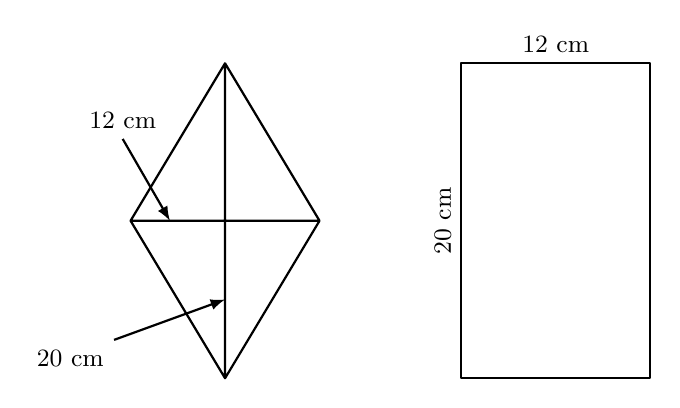
\begin{tikzpicture}[scale=1,line width=0.8pt,line join=round,>=stealth]
			\def\a{4} 	\def\b{2.4} 
			\path (0,0) coordinate (A)
			(A)+(-90:\a) coordinate (C)
			(A)+(-\b/2,-\a/2) coordinate (B)
			(B)+(0:\b) coordinate (D)
			;
			\draw[latex-] (B)++(0:0.5)--++(120:0.5*\b)node[above]{\small 12 cm} ;
			\draw[latex-] (C)++(90:1)--++(-160:1.5)node[below left]{\small 20 cm} ;
			\draw (A)--(B)--(C)--(D)--(A)--(C) (B)--(D);
			\draw (3,0)--++(0:\b)node[above,midway]{\small 12 cm}--++(-90:\a)--++(180:\b)--cycle node[sloped,above,midway]{\small 20 cm};
		\end{tikzpicture}
	}
	
\end{ex}


\begin{ex}
	Một thửa ruộng hình chữ nhật có chiều dài 	là 24 m, chiều rộng 18 m. Trên thửa ruộng đó, mỗi 
	mét vuông thu hoạch được 5 kg rau. Hỏi cả thửa 	ruộng đó thu hoạch được bao nhiêu ki – lô – gam 
	rau? 
	
	\choice
	{432 kg}
	{\True 2160 kg}
	{518 kg}
	{1080 kg}
	
\end{ex}

\begin{ex}%[6H1B2-4] 
	Một nền nhà hình chữ nhật có chiều dài 20 m và chiều rộng bằng $\frac{1}{4}$ chiều dài. Người ta muốn lát gạch hình vuông cạnh 5 dm lên nền nhà đó nên đã mua gạch với tổng số tiền là $36\,800\,000$ đồng (giả sử khoảng cách giữa hai viên gạch kề nhau là không đáng kể). Hỏi giá của một viên gạch là bao nhiêu?
	\choice
	{ $90\,000$ đồng}
	{ $91\,000$ đồng)}
	{\True $92\,000$ đồng}
	{$93\,000$ đồng}
\end{ex}

%%=====Câu 55
\begin{ex}\immini[thm]{
	Tính diện tích hình bên:
	\choice
	{180 m}
	{1550 m}
	{\True 1550 m$^ 2$}
	{ 180 m$^2$}	
	}{\begin{tikzpicture}[scale=1,line width=0.8pt,line join=round,>=stealth]
		\def\sc{15} 
		\path (0,0) coordinate (A)
		(A)+(15/\sc,20/\sc) coordinate (B)
		(B)+(40/\sc,30/\sc) coordinate (C)
		(B)+(0:40/\sc) coordinate (D)
		(A)+(0:55/\sc) coordinate (E)
		;
		\draw[latex-latex,dashed] (A)++(180:0.3)--++(90:20/\sc)node[midway,left]{\small 20 cm} ;
		\draw[latex-latex,dashed] (C)++(0:0.6)--++(-90:50/\sc)node[midway,right]{\small 50 cm} ;
		\draw[latex-latex,dashed] (C)++(90:0.3)--++(180:40/\sc)node[midway,above]{\small 40 cm} ;
		\draw (A)--(B)node[midway,above,sloped]{\small 25 cm}
		--(C)node[midway,above,sloped]{\small 50 cm}
		--(E)--(A)node[midway,below]{\small 55 cm} (B)--(D);
		\draw[dashed] (B)--++(180:15/\sc+0.3)
			(B)--++(90:30/\sc+0.3);
		\foreach \x/ \goc in {A/-90,B/135,C/0,D/0,E/-45}  \fill (\x) circle (1.5pt)	
				($(\x)+(\goc:3mm)$) node {$\x$};
	\end{tikzpicture}	
	}
\end{ex}



%%=====Câu 59
\begin{ex}\immini[thm]{
	Cho hình chữ nhật $ABFE$ và hình thoi $ABCD$, biết $CD=5$ cm và $AE=2$ cm. Diện tích của hình chữ nhật $ABFE$ bằng:
	\choice
	{14 cm$^2$}
	{7 cm$^2$}
	{\True 10 cm$^2$}
	{5 cm$^2$}	
	}{
	\begin{tikzpicture}[scale=1,line width=0.8pt,line join=round,>=stealth]
		\def\a{2.5} 	\def\b{1} 	\def\g{20} 
		\path (0,0) coordinate (A)
		(A)+(\g-180:\a) coordinate (B)
		(B)+(-\g:\a) coordinate (C)
		(C)+(\g:\a) coordinate (D)
		(A)+(90+\g:\b) coordinate (E)
		(E)+(B) coordinate (F)
		;
		\draw[latex-latex] (A)++(\g:0.3)--++(90+\g:\b)node[midway,right]{\small 2 cm} ;
		\draw[latex-latex] (C)++(\g-90:0.3)--++(\g:\a)node[midway,below,sloped]{\small 5 cm} ;
		\draw (A)--(B)--(C)--(D)--(A)--(E)--(F)--(B);
		\foreach \x/ \goc in {A/160,B/200,C/-120,D/30,E/90,F/160}  \fill (\x) circle (1.5pt)	
		($(\x)+(\goc:3mm)$) node {$\x$};
	\end{tikzpicture}
	}
	
\end{ex}


